\documentclass[11pt]{article}
\usepackage[margin=2.5cm]{geometry}
\usepackage{booktabs}
\usepackage{tabularx}
\usepackage{graphicx}
\usepackage[hidelinks]{hyperref}
\usepackage{times}
\usepackage{enumitem}
\usepackage{float}
\usepackage{amsmath}
\usepackage{tikz}
\usetikzlibrary{positioning}
\tikzset{
  fsub/.style={circle, draw=blue!70!black, fill=blue!45, minimum size=5mm, inner sep=0},
  fgray/.style={circle, draw=gray, fill=gray!20, minimum size=5mm, inner sep=0},
  forange/.style={circle, draw=orange!80!black, fill=orange!50, minimum size=5mm, inner sep=0},
  fgreen/.style={circle, draw=green!50!black, fill=green!40, minimum size=5mm, inner sep=0},
  fbox/.style={draw, rounded corners=3pt, align=center, font=\footnotesize},
  fedge/.style={gray!70, thick},
  farrow/.style={-latex, thick},
  ftitle/.style={font=\small\bfseries},
  fnote/.style={font=\footnotesize, align=center}}

% Small example graph for the GLASS figure. Inside nodes: a, b, c.
\newcommand{\glassgraph}[2]{%
  \node[#1] (a) at (0,1)    {};
  \node[#1] (b) at (1,1.6)  {};
  \node[#1] (c) at (1,0.4)  {};
  \node[#2] (d) at (2,1.6)  {};
  \node[#2] (e) at (2,0.4)  {};
  \node[#2] (f) at (-0.9,1.7) {};
  \node[#2] (g) at (-0.9,0.3) {};
  \draw[edge] (a)--(b) (a)--(c) (b)--(c) (b)--(d) (c)--(e) (d)--(e) (a)--(f) (a)--(g) (f)--(g);
}
\setlist[description]{leftmargin=2.2cm, labelwidth=2.0cm, itemsep=2pt, font=\normalfont\itshape}

\title{Subgraph Representation Learning:\\ The Main Methods}
\author{}
\date{October 13, 2026}

\begin{document}
\maketitle

\section*{The problem}

There is one large graph. A \emph{subgraph} is a set of its nodes, for example the visits of
one patient. Each subgraph has a label, and the task is to predict it. Methods for this task
are called \emph{subgraph representation learning}: they turn each subgraph into one vector,
and a classifier reads the label from that vector.

The task sits between two better-known ones. In \emph{node classification} the thing to label
is a single node. In \emph{graph classification} it is a whole small graph, such as a molecule,
that stands alone. Here the thing to label is a group of nodes that lives inside one big graph,
so the nodes and edges around it can matter as much as the nodes in it.

\paragraph{Why a plain GNN is not enough.} The simple approach is to run a graph neural network
(GNN) on the whole graph, which gives every node a vector, and then average the vectors of the
subgraph's nodes. The weakness is that the GNN does not know which nodes belong to the
subgraph. A node's vector is the same whichever subgraph we are asking about, so the model
cannot tell a neighbour inside the subgraph from one outside it. Most methods below are ways
around this, or ways to do it more cheaply.

\section*{The methods at a glance}

\begin{table}[H]
\centering
\small
\begin{tabularx}{\textwidth}{llX}
\toprule
Method & Where, year & Main idea \\
\midrule
SubGNN & NeurIPS 2020 & Messages to each subgraph from sampled small patches of the graph, in three channels: position, neighbourhood and structure. \\
GLASS & ICLR 2022 & Mark every node as inside or outside the subgraph, then run a plain GNN that treats the two kinds differently. \\
S2N & ICML 2024 & Turn every subgraph into one node of a new small graph, then run a simple GNN on it. \\
GPEN & ICML 2025 & Give each node a position in a tree over the whole graph, so far-away structure is used. \\
\bottomrule
\end{tabularx}
\caption{The main methods, oldest first.}
\end{table}

\section*{Each method}

\paragraph{SubGNN (Alsentzer et al.)} The first method, and the source of the standard
datasets. It compares each subgraph with small random pieces of the graph, and asks three
questions: where the subgraph sits, what is around it, and what shape it has. It is slow,
because the pieces must be prepared in advance.

\begin{figure}[H]
\centering
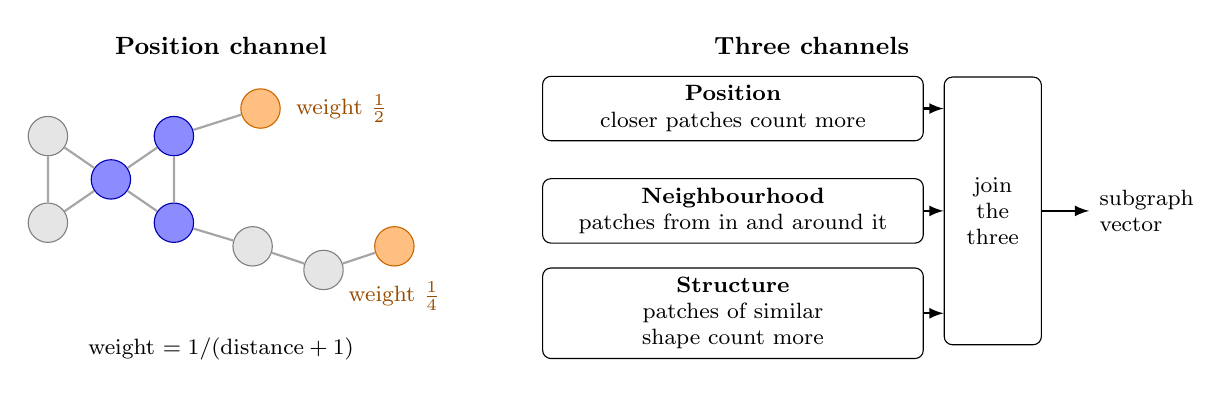
\begin{tikzpicture}
  % Left: the position channel on a small graph
  \node[fgray]   (y1) at (-0.8,0.95) {};
  \node[fgray]   (y2) at (-0.8,-0.15) {};
  \node[fsub]    (s1) at (0,0.4) {};
  \node[fsub]    (s2) at (0.8,0.95) {};
  \node[fsub]    (s3) at (0.8,-0.15) {};
  \node[forange] (pn) at (1.9,1.3) {};
  \node[fgray]   (x1) at (1.8,-0.45) {};
  \node[fgray]   (x2) at (2.7,-0.75) {};
  \node[forange] (pf) at (3.6,-0.45) {};
  \draw[fedge] (s1)--(s2) (s1)--(s3) (s2)--(s3) (s2)--(pn) (s3)--(x1) (x1)--(x2) (x2)--(pf)
               (s1)--(y1) (s1)--(y2) (y1)--(y2);
  \node[font=\footnotesize, text=orange!60!black, right=2pt of pn] {weight $\tfrac12$};
  \node[font=\footnotesize, text=orange!60!black, below=2pt of pf] {weight $\tfrac14$};
  \node[ftitle] at (1.4,2.1) {Position channel};
  \node[fnote] at (1.4,-1.75) {weight $= 1/(\text{distance}+1)$};

  % Right: the three channels
  \node[ftitle] at (8.9,2.1) {Three channels};
  \node[fbox, text width=46mm] (cp) at (7.9,1.3)  {\textbf{Position}\\ closer patches count more};
  \node[fbox, text width=46mm] (cn) at (7.9,0)    {\textbf{Neighbourhood}\\ patches from in and around it};
  \node[fbox, text width=46mm] (cs) at (7.9,-1.3) {\textbf{Structure}\\ patches of similar shape count more};
  \node[fbox, minimum height=34mm, text width=10mm] (join) at (11.2,0) {join\\ the\\ three};
  \draw[farrow] (cp.east) -- (join.west |- cp);
  \draw[farrow] (cn.east) -- (join.west |- cn);
  \draw[farrow] (cs.east) -- (join.west |- cs);
  \draw[farrow] (join.east) -- ++(0.6,0) node[right, fnote, align=left] {subgraph\\ vector};
\end{tikzpicture}
\caption{How SubGNN works. Left: orange patches send messages to the blue subgraph. A patch
one step away gets weight $\tfrac12$, a patch three steps away gets $\tfrac14$. Right: the
same idea in three channels, each with its own patches and its own weight. Each channel is run
twice, for the inside of the subgraph and for its border. Patches and weights are computed
before training.}
\end{figure}

\paragraph{GLASS (Wang and Zhang)} It tells the GNN which nodes are in the subgraph: each node
gets a mark, $1$ inside and $0$ outside. The GNN treats the two kinds differently, so the same
node can look different for different subgraphs. Simpler and faster than SubGNN, and better on
all datasets.

\begin{figure}[H]
\centering
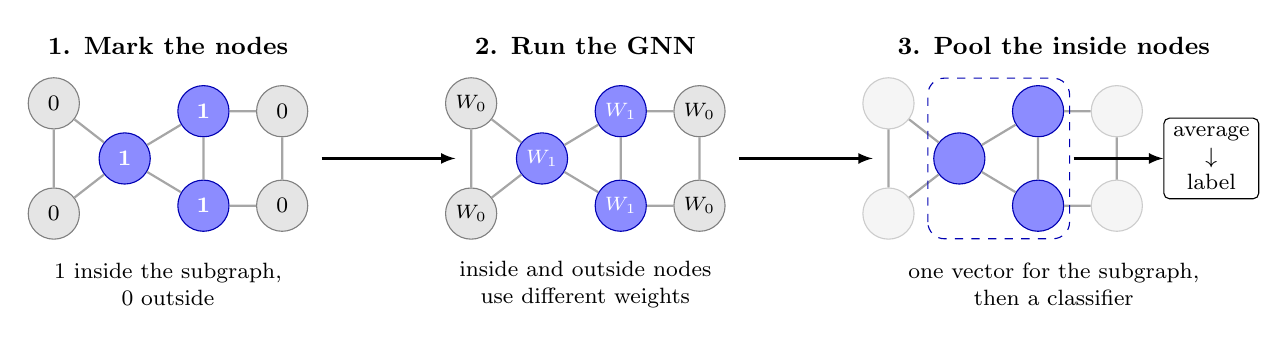
\begin{tikzpicture}[
  every node/.style={font=\small},
  innode/.style={circle, draw=blue!70!black, fill=blue!45, minimum size=6.5mm, inner sep=0},
  outnode/.style={circle, draw=gray, fill=gray!20, minimum size=6.5mm, inner sep=0},
  faded/.style={circle, draw=gray!40, fill=gray!8, minimum size=6.5mm, inner sep=0},
  edge/.style={gray!70, thick},
  title/.style={font=\small\bfseries, anchor=south},
  arrow/.style={-latex, thick}]

  % 1. Mark the nodes
  \begin{scope}
    \glassgraph{innode}{outnode}
    \foreach \n in {a,b,c} \node[white, font=\footnotesize\bfseries] at (\n) {1};
    \foreach \n in {d,e,f,g} \node[font=\footnotesize] at (\n) {0};
    \node[title] at (0.55,2.2) {1. Mark the nodes};
    \node[align=center, font=\footnotesize] at (0.55,-0.6) {$1$ inside the subgraph,\\ $0$ outside};
  \end{scope}

  % 2. Run the GNN
  \begin{scope}[xshift=5.3cm]
    \glassgraph{innode}{outnode}
    \foreach \n in {a,b,c} \node[white, font=\scriptsize] at (\n) {$W_1$};
    \foreach \n in {d,e,f,g} \node[font=\scriptsize] at (\n) {$W_0$};
    \node[title] at (0.55,2.2) {2. Run the GNN};
    \node[align=center, font=\footnotesize] at (0.55,-0.6) {inside and outside nodes\\ use different weights};
  \end{scope}

  % 3. Pool the inside nodes
  \begin{scope}[xshift=10.6cm]
    \glassgraph{innode}{faded}
    \draw[blue!70!black, dashed, rounded corners=6pt] (-0.4,-0.02) rectangle (1.4,2.02);
    \node[draw, rounded corners=2pt, fill=white, align=center, font=\footnotesize] (pool) at (3.2,1) {average\\ $\downarrow$\\ label};
    \draw[arrow] (1.45,1) -- (pool.west);
    \node[title] at (1.2,2.2) {3. Pool the inside nodes};
    \node[align=center, font=\footnotesize] at (1.2,-0.6) {one vector for the subgraph,\\ then a classifier};
  \end{scope}

  \draw[arrow] (2.5,1) -- (4.2,1);
  \draw[arrow] (7.8,1) -- (9.5,1);
\end{tikzpicture}
\caption{How GLASS works. Blue nodes are the subgraph. The marks change for every subgraph,
so the GNN runs again for each one (or for each batch of subgraphs).}
\end{figure}

\begin{figure}[H]
\centering
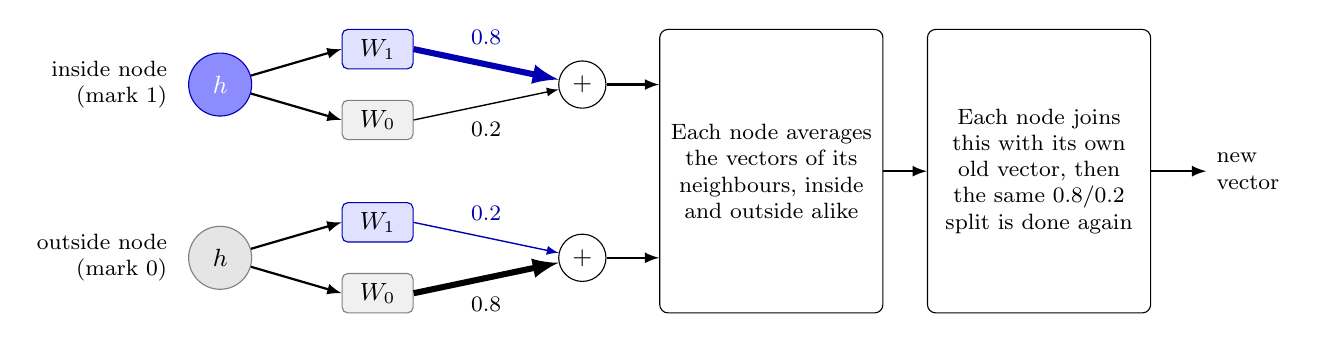
\begin{tikzpicture}[
  every node/.style={font=\small},
  vin/.style={circle, draw=blue!70!black, fill=blue!45, minimum size=8mm, inner sep=0},
  vout/.style={circle, draw=gray, fill=gray!20, minimum size=8mm, inner sep=0},
  w1/.style={draw=blue!70!black, fill=blue!12, rounded corners=2pt, minimum width=9mm, minimum height=5mm},
  w0/.style={draw=gray, fill=gray!12, rounded corners=2pt, minimum width=9mm, minimum height=5mm},
  mix/.style={circle, draw, minimum size=6mm, inner sep=0, font=\small},
  stepbox/.style={draw, rounded corners=3pt, align=center, font=\footnotesize, minimum height=36mm, text width=26mm},
  heavy/.style={-latex, line width=2.2pt},
  light/.style={-latex, line width=0.5pt},
  arrow/.style={-latex, thick},
  w/.style={font=\footnotesize, fill=white, inner sep=1pt}]

  % Inside node
  \node[vin]  (hin)  at (0, 1.1)  {\textcolor{white}{$h$}};
  \node[w1]   (a1)   at (2, 1.55) {$W_1$};
  \node[w0]   (a0)   at (2, 0.65) {$W_0$};
  \node[mix]  (min)  at (4.6, 1.1)  {$+$};
  \draw[arrow] (hin) -- (a1.west);
  \draw[arrow] (hin) -- (a0.west);
  \draw[heavy, blue!70!black] (a1.east) -- node[w, above=5pt] {$0.8$} (min);
  \draw[light] (a0.east) -- node[w, below=5pt] {$0.2$} (min);
  \node[font=\footnotesize, anchor=east, align=right] at (-0.55,1.1) {inside node\\(mark $1$)};

  % Outside node
  \node[vout] (hout) at (0,-1.1)  {$h$};
  \node[w1]   (b1)   at (2,-0.65) {$W_1$};
  \node[w0]   (b0)   at (2,-1.55) {$W_0$};
  \node[mix]  (mout) at (4.6,-1.1)  {$+$};
  \draw[arrow] (hout) -- (b1.west);
  \draw[arrow] (hout) -- (b0.west);
  \draw[light, blue!70!black] (b1.east) -- node[w, above=5pt] {$0.2$} (mout);
  \draw[heavy] (b0.east) -- node[w, below=5pt] {$0.8$} (mout);
  \node[font=\footnotesize, anchor=east, align=right] at (-0.55,-1.1) {outside node\\(mark $0$)};

  % Rest of the layer
  \node[stepbox] (avg) at (7.0,0) {Each node averages\\ the vectors of its\\ neighbours, inside\\ and outside alike};
  \node[stepbox] (comb) at (10.4,0) {Each node joins\\ this with its own\\ old vector, then\\ the same $0.8$/$0.2$\\ split is done again};
  \draw[arrow] (min) -- (avg.west |- min);
  \draw[arrow] (mout) -- (avg.west |- mout);
  \draw[arrow] (avg) -- (comb);
  \draw[arrow] (comb.east) -- ++(0.7,0) node[right, align=left, font=\footnotesize] {new\\ vector};
\end{tikzpicture}
\caption{One GLASS layer, as written in the authors' code. Every node goes through both weight
sets, $W_1$ and $W_0$. The mark only decides the mix: inside nodes take mostly $W_1$, outside
nodes mostly $W_0$. The $0.8$ is a fixed setting, not learned. The mark is not given to the
network as a feature; this split is the only place it is used.}
\end{figure}

\paragraph{S2N (Kim and Oh)} It turns each subgraph into one node of a new, small graph, and
joins two such nodes when their subgraphs are linked. A plain GNN then labels the nodes of
this small graph. As good as GLASS, and $183$ to $711$ times faster.

\begin{figure}[H]
\centering
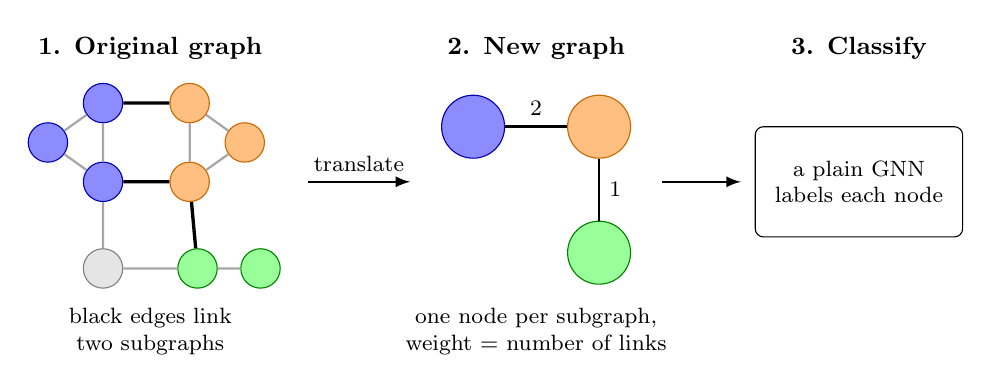
\begin{tikzpicture}
  % Left: original graph with three subgraphs
  \node[fsub]    (b1) at (0,1.0) {};
  \node[fsub]    (b2) at (0.7,1.5) {};
  \node[fsub]    (b3) at (0.7,0.5) {};
  \node[forange] (o1) at (1.8,1.5) {};
  \node[forange] (o2) at (1.8,0.5) {};
  \node[forange] (o3) at (2.5,1.0) {};
  \node[fgreen]  (g1) at (1.9,-0.6) {};
  \node[fgreen]  (g2) at (2.7,-0.6) {};
  \node[fgray]   (n1) at (0.7,-0.6) {};
  \draw[fedge] (b1)--(b2) (b1)--(b3) (b2)--(b3) (o1)--(o2) (o1)--(o3) (o2)--(o3) (g1)--(g2)
               (b3)--(n1) (n1)--(g1);
  \draw[very thick] (b2)--(o1) (b3)--(o2) (o2)--(g1);
  \node[ftitle] at (1.3,2.2) {1. Original graph};
  \node[fnote] at (1.3,-1.4) {black edges link\\ two subgraphs};

  \draw[farrow] (3.3,0.5) -- node[above, fnote] {translate} (4.6,0.5);

  % Middle: new graph, one node per subgraph
  \node[fsub,    minimum size=8mm] (A) at (5.4,1.2) {};
  \node[forange, minimum size=8mm] (B) at (7.0,1.2) {};
  \node[fgreen,  minimum size=8mm] (C) at (7.0,-0.4) {};
  \draw[very thick] (A) -- node[above, fnote] {$2$} (B);
  \draw[thick] (B) -- node[right, fnote] {$1$} (C);
  \node[ftitle] at (6.2,2.2) {2. New graph};
  \node[fnote] at (6.2,-1.4) {one node per subgraph,\\ weight $=$ number of links};

  \draw[farrow] (7.8,0.5) -- (8.8,0.5);

  % Right: GNN
  \node[fbox, text width=24mm, minimum height=14mm] at (10.3,0.5) {a plain GNN\\ labels each node};
  \node[ftitle] at (10.3,2.2) {3. Classify};
\end{tikzpicture}
\caption{How S2N works. Each subgraph becomes one node. Two new nodes are joined when edges
link their subgraphs, and the edge weight is the number of such edges. Blue and green are
linked only through a gray node, so they get no edge. Each new node starts from a weighted sum
of its nodes' features, or from a small GNN run on the subgraph alone.}
\end{figure}

\paragraph{GPEN (Wu et al.)} It adds information from far away in the graph. It builds one
tree over the whole graph and gives each node a position: its distance from the root. The
newest method, and the best on all four real datasets.

\begin{figure}[H]
\centering
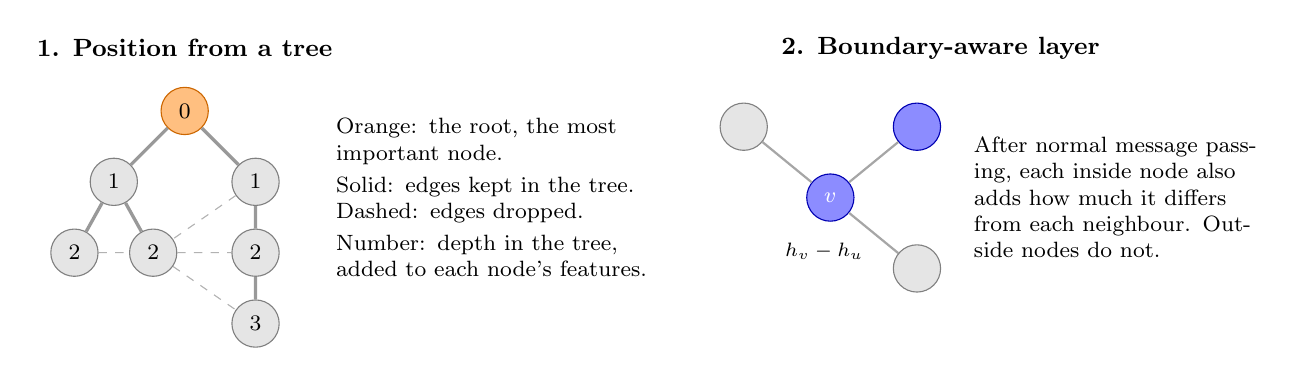
\begin{tikzpicture}
  % Left: tree positions
  \node[forange, minimum size=6mm] (r) at (0,1.4)    {\footnotesize 0};
  \node[fgray,   minimum size=6mm] (a) at (-0.9,0.5) {\footnotesize 1};
  \node[fgray,   minimum size=6mm] (b) at (0.9,0.5)  {\footnotesize 1};
  \node[fgray,   minimum size=6mm] (c) at (-1.4,-0.4) {\footnotesize 2};
  \node[fgray,   minimum size=6mm] (d) at (-0.4,-0.4) {\footnotesize 2};
  \node[fgray,   minimum size=6mm] (e) at (0.9,-0.4)  {\footnotesize 2};
  \node[fgray,   minimum size=6mm] (f) at (0.9,-1.3)  {\footnotesize 3};
  \draw[very thick, gray!80] (r)--(a) (r)--(b) (a)--(c) (a)--(d) (b)--(e) (e)--(f);
  \draw[gray!60, dashed] (c)--(d) (d)--(e) (b)--(d) (d)--(f);
  \node[ftitle] at (0,2.2) {1. Position from a tree};
  \node[fnote, anchor=west, text width=40mm, align=left] at (1.8,0.3)
    {Orange: the root, the most important node.\\[2pt]
     Solid: edges kept in the tree.\\ Dashed: edges dropped.\\[2pt]
     Number: depth in the tree, added to each node's features.};

  % Right: boundary-aware layer
  \node[fsub,  minimum size=6mm] (v)  at (8.2,0.3) {\footnotesize\textcolor{white}{$v$}};
  \node[fsub,  minimum size=6mm] (u1) at (9.3,1.2) {};
  \node[fgray, minimum size=6mm] (u2) at (9.3,-0.6) {};
  \node[fgray, minimum size=6mm] (u3) at (7.1,1.2) {};
  \draw[fedge] (v)--(u1) (v)--(u3);
  \draw[fedge] (v) -- node[below left=0pt, font=\scriptsize, text=black] {$h_v - h_u$} (u2);
  \node[ftitle] at (9.6,2.2) {2. Boundary-aware layer};
  \node[fnote, anchor=west, text width=36mm, align=left] at (9.9,0.3)
    {After normal message passing, each inside node also adds how much it differs from each
     neighbour. Outside nodes do not.};
\end{tikzpicture}
\caption{How GPEN works. Left: nodes are scored by importance (similar to PageRank), the top
node becomes the root, and a tree is built from the strongest edges. Each node's depth is
added to its features. Right: for an inside node $v$, the layer output is
$(1-\beta)\,h_v + \beta \sum_u (h_v - h_u)$, summed over its neighbours $u$. For an outside node
it is $(1-\beta)\,h_v$. $\beta$ is a fixed setting.}
\end{figure}

\section*{Published results}

\begin{table}[H]
\centering
\small
\begin{tabular}{lrrrr}
\toprule
 & PPI-BP & HPO-Metab & HPO-Neuro & EM-User \\
\midrule
SubGNN & $59.9 \pm 2.5$ & $53.7 \pm 2.5$ & $64.4 \pm 1.9$ & $81.6 \pm 4.1$ \\
GLASS & $61.9 \pm 2.2$ & $61.4 \pm 1.6$ & $68.5 \pm 1.6$ & $88.8 \pm 1.9$ \\
S2N & $64.3 \pm 4.1$ & $\mathbf{63.9 \pm 7.2}$ & $68.6 \pm 1.9$ & $89.0 \pm 3.5$ \\
GPEN & $\mathbf{64.4 \pm 0.9}$ & $\mathbf{63.9 \pm 0.9}$ & $\mathbf{69.1 \pm 0.6}$ & $\mathbf{91.2 \pm 1.3}$ \\
\bottomrule
\end{tabular}
\caption{Real datasets. Micro-F1 on the test set, mean and spread over $10$ runs, from
Table 1 of the GPEN paper. For the binary EM-User this is the accuracy.}
\end{table}

\begin{table}[H]
\centering
\small
\begin{tabular}{lrrrr}
\toprule
 & Density & Cut ratio & Coreness & Component \\
\midrule
SubGNN & $91.9 \pm 1.9$ & $62.9 \pm 4.1$ & $65.9 \pm 9.8$ & $95.8 \pm 10.1$ \\
GLASS & $93.0 \pm 2.8$ & $93.5 \pm 1.9$ & $84.0 \pm 2.8$ & $\mathbf{100.0 \pm 0.0}$ \\
S2N & $\mathbf{96.3 \pm 5.7}$ & $89.2 \pm 4.4$ & $72.6 \pm 11.4$ & $\mathbf{100.0 \pm 0.0}$ \\
GPEN & $95.6 \pm 1.6$ & $\mathbf{93.6 \pm 1.6}$ & $\mathbf{87.6 \pm 1.9}$ & $\mathbf{100.0 \pm 0.0}$ \\
\bottomrule
\end{tabular}
\caption{Synthetic datasets. Micro-F1 on the test set, mean and spread over $10$ runs, from
Table 3 of the GPEN paper.}
\end{table}

\section*{What the methods have in common}

\paragraph{Everyone uses the same datasets.} SubGNN, GLASS, S2N and GPEN all report on
SubGNN's four real datasets and its four synthetic ones. Only one of the real ones, EM-User,
has a binary label.

\paragraph{Knowing what is inside matters.} GLASS showed that just marking the subgraph's
nodes lifts a plain GNN by a large margin, to more than double the score on one dataset. Most later
methods either keep this idea or find another way to give the model the same information.

\paragraph{Cost is the second big topic.} SubGNN needs heavy precomputation, and GLASS must
run the GNN again for each small batch of subgraphs, because the marks change with the batch.
S2N was made mainly to be cheaper.

\paragraph{Gains have become small.} On the real datasets, from GLASS to GPEN the best scores
moved by at most $2.5$ points. GPEN beats S2N by at most $2.2$ points, which is less than the
spread of S2N's runs. On the synthetic datasets, Component is solved by all three newer
methods, and the only clear gap left is on Coreness, where GPEN leads GLASS by $3.6$ points.

\end{document}
